\documentclass{article} % This line defines the type of document. 'article' is a common class for small documents.
\usepackage[margin=1.4in]{geometry}
\usepackage{graphicx}
\usepackage{titlesec}
\usepackage{caption}
% \usepackage{hyperref}
\usepackage[colorlinks=true, linkcolor=blue, citecolor=blue, urlcolor=blue]{hyperref}


% Set paragraph indentation to zero
\setlength{\parindent}{0pt}

\titleformat{\section}
  {\normalfont\large\bfseries}{\thesection}{1em}{}

\begin{document} % This line marks the beginning of the document content.


\noindent\makebox[\linewidth]{\rule{\textwidth}{1pt}} 
\vspace*{0mm} % adds vertical space before the title
\begin{center}
    \Large\textbf{Toy Models of Superposition Replication and Findings}
\end{center}
\vspace*{2mm} % adds vertical space before the title
\noindent\makebox[\linewidth]{\rule{\textwidth}{1pt}}
\newline

\begin{abstract}
\begin{quote}
    Toy Models of Superpostion\cite{elhage2022toy} is a groundbreaking paper published by 
    researchers affilated with Anthropic and Harvard University in 2022. By 
    investigating small models with under 100 neurons, the paper demonstrates 
    that neural networks can represent more features than they have demensions. 
    Additionally, they use these so called "toy models" to understand the 
    relationship between how neural networks are trained and how they represent 
    the data internally. This paper was able to the finding from this paper and 
    make new observations about "toy models" and how they behave under different 
    training circumstances.
\end{quote}
\end{abstract}


\section{Introduction}

The orginal paper motivates the idea of superpostion with the following graphic:

\begin{figure}[h]
    \centering
    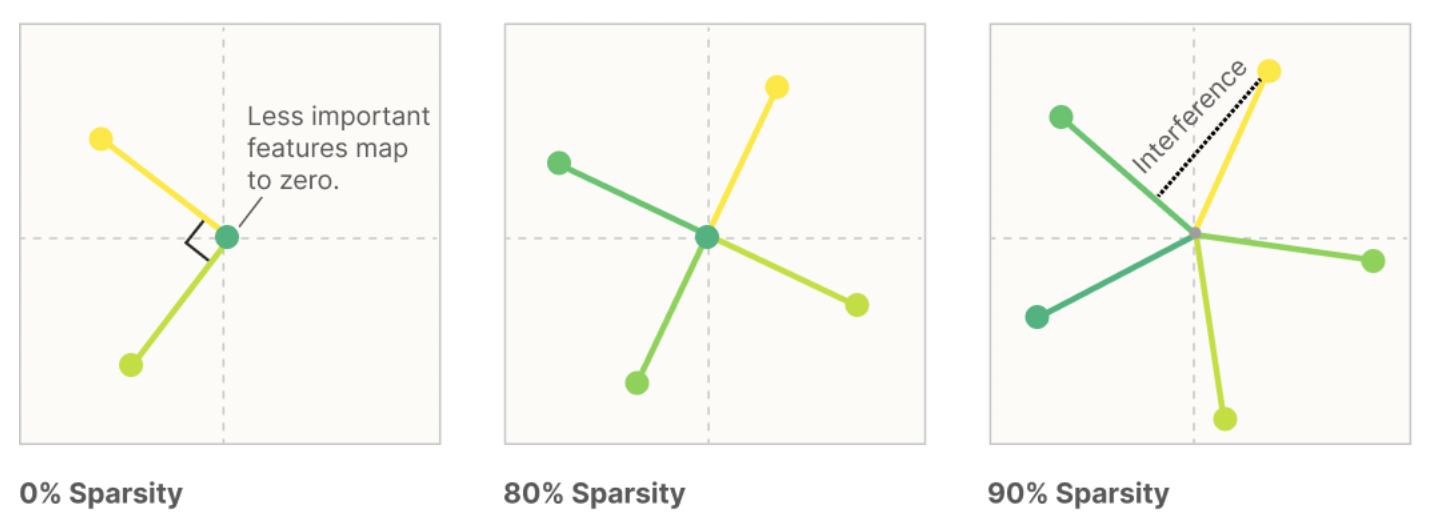
\includegraphics[width=0.61\linewidth]{section_1/images/section1_anthropic_graphic_.png}
    \captionsetup{font=footnotesize} % Set the font size for this caption
    % \caption{Graphic from Anthropic Paper}
    \label{fig:section1_anthropic}
\end{figure}
The basic idea is this: if you think of each feature as being represented inside a
nueral network as a direction, you can graph these directions and observe them.
In the graphic above, the researchers studied a model with two neurons and five inputs.
Recreating this model showed the same results when sparsity was varied. A replication
of the original graphic can be found below and the code used to generate it can be found \href{http://www.example.com}{here}. 

\begin{figure}[h]
    \centering
    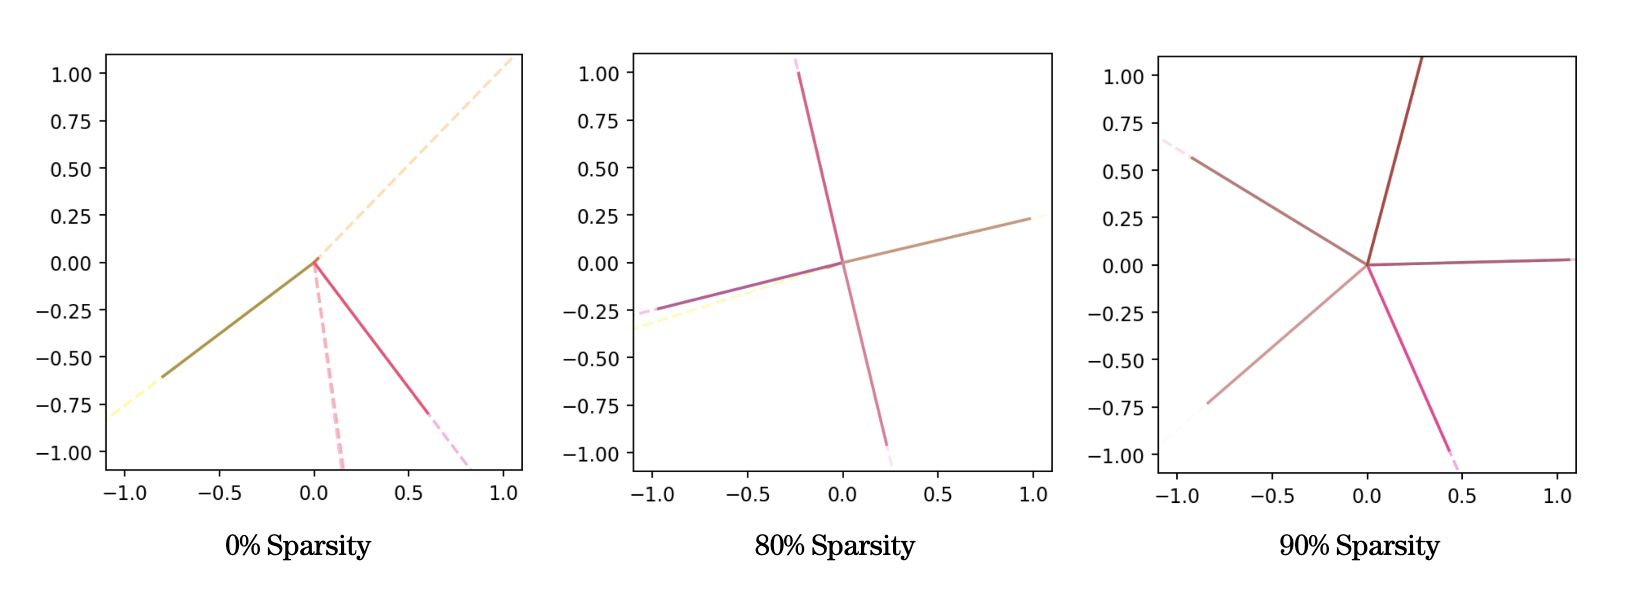
\includegraphics[width=0.68\linewidth]{section_1/images/section1_replicated_graphic.png}
    \captionsetup{font=footnotesize} % Set the font size for this caption
    % \caption{Replicated feature directions example.}
    \label{fig:section1_replication}
\end{figure}

Although this example only has two neurons (meaning it can be graphed in 2D), in
future sections we will see how similar aproachs scale nicely to models with more neurons.
As far as I understand, it is still unclear weather the ideas 
dicussed in the original paper can be scaled to help understand and identify bias in 
much larger models such as GTP-4, Claude 2, or Gemini.



\section{Background and Motivation}

In this section of Toy Models of Superpostion\cite{elhage2022toy}, the authors
provide context and define terms.  In this paper, I make a few additional comments 
about some of the key ideas and terms the authors discuss. \newline \newline
\textbf{(1) Defining Features: }The original paper Toy Models of Superpostion
defines features broadly as "properties of the input which a sufficiently large 
neural network will reliably dedicate a neuron to representing." The authors do
however describe this definition as "slightly circular" and note that they are
not "overly attached to it." I find the definition especially problematic because a network that is small or
has unconventional archetecture may represent a feature that a larger network
or a network with a more typical archetecture may represent. These 
representations are clearly still features, but are not treated as so under the
original definition.\newline\newline
As a result, I propose an alternative definition: features are aspects of the
input that a neural network represents accuratly with a higher propability than 
a randomly initialized network. In other words, features are parts of the input 
that a model determines to be important enough to represent internally.\newline\newline
\textbf{(2) Role of linear functions in Neural Networks: }The original authors of
Toy Models of Superpostion strongly emphasize the role of linear functions in
neural networks. They claim that "Linear representations are the natural format 
for neural networks to represent information in!" Although this is clearly 
mostly true, I dont think there is sufficient evidence to justify the confidence 
of the authors in the original paper. Nonlinearities are also clearly doing lots 
of useful computation and it seems just as important to study their role in how 
a neural network represents features from layer to layer. The nonlinearity at 
each layer of a neural network may be just as important as the linear 
transformation in understanding how a model makes decisions.\newline\newline
\textbf{(3) Defining Superposition: } The original paper has a fantastic and
simple defination for Superposition: "Roughly, the idea of 
superposition is that neural networks 'want to represent more features than they 
have neurons', so they exploit a property of high-dimensional spaces to 
simulate a model with many more neurons." This is the definition I will used
throughout this paper.

\section{Demonstrating Superposition}

\bibliographystyle{plain}
\bibliography{references}

\end{document} % This line marks the end of the document content.
